% Preamble
\documentclass[11pt]{amsart}
\usepackage{mathtools}
\usepackage{amssymb,latexsym}
\usepackage{physics}
\usepackage{listings}
\usepackage{bm}
\usepackage{enumerate}
\usepackage{graphicx}
\usepackage{placeins}
\usepackage{color}
\usepackage{hyperref}
\usepackage{pgf,tikz}
\usepackage{mathrsfs}
\usetikzlibrary{arrows}

% Environments
\theoremstyle{definition}
\newtheorem{theorem}{Theorem}
\newtheorem{algorithm}{Algorithm}
\newtheorem{corollary}{Corollary}
\newtheorem*{main}{Main Theorem}
\newtheorem{lemma}{Lemma}[section]
\newtheorem{proposition}{Proposition}
\newtheorem{definition}{Definition}
\newtheorem{example}{Example}
\theoremstyle{remark}
\newtheorem*{notation}{Notation}

% Commands and operators
\newcommand{\ind}{\hspace*{0.5cm}}
\newcommand{\gap}{\hspace*{0.25cm}}
\newcommand*{\Cdot}{\raisebox{-0.25ex}{\scalebox{1.3}{$\cdot$}}}
\newcommand{\vect}[1]{\mathbf{#1}}
\newcommand{\transpose}{T}
\DeclareMathOperator{\interior}{\textbf{int}}
\DeclareMathOperator{\domain}{\textbf{dom}}
\DeclareMathOperator{\diag}{\textbf{diag}}
\DeclareMathOperator{\sign}{\textbf{sign}}
\DeclareMathOperator{\CG}{\textbf{CG}}
\DeclareMathOperator{\vol}{\textbf{vol}}
\DeclareMathOperator{\CC}{\textbf{CC}}
\DeclareMathOperator{\AC}{\textbf{AC}}
\DeclareMathOperator{\centerr}{\textbf{center}}

\begin{document}
\lstset{language=}
\pagestyle{plain}

\title{Cutting-plane methods with applications in convex optimization and active learning}
\author{David Wu}

\maketitle

% \tableofcontents

\section{Introduction}

    \subsection{Outline.}
        In this report we present a general cutting-plane algorithm for the problem of finding a point in a target set contained in a bounded convex polyhedron. We then show how this general algorithm can be specialized to (i) solve convex optimization problems, giving the so-called analytic center cutting plane method (ACCPM); and (ii) solve an active learning problem in the context of binary linear classification. Crucial to these algorithms is finding the approximate center of a bounded convex polyhedron. The center of a bounded convex polyhedron has no clear definition, so we present several definitions from the literature: (i) the analytic center (AC); (ii) the Chebyshev center (CC); and (iii) the center of gravity (CG). The AC and CC are used in the algorithms we present while the CG is of theoretical interest. Therefore, we explain how the AC and CC can be computed. Furthermore, we present an experiment involving training logistic regression using the ACCPM and several experiments involving the active learning algorithm on real data. The code and notebooks corresponding to this report can be found in the project's GitHub repository \footnote{The GitHub repository is \url{https://github.com/davidjwu/mclass-sky/tree/master/projects/david}}.

    \subsection{Related and background works.}
        Our exposition of the material on the general cutting-plane algorithm, computing the AC and ACCPM closely follows notes on the topic by S. Boyd et al. \cite{BVS08} \cite{BV11} \cite{BDV15}. S. Boyd's textbook on convex optimization \cite{BV04} was an invaluable source for background knowledge also. Our exposition of the material on active learning closely follows a paper by U. Louche and L. Ralaivola \cite{LR15}.

    \subsection{Notation and conventions}
        Throughout this paper (unless otherwise stated) we will use the following notation and conventions: 
        \begin{itemize}
            \item we use the notation $Ax \preceq b$ to represent a system of $m$ linear inequalities $a_i^\transpose x \leq b, i = 1, \dots, m$. Therefor the rows of $A$ and entries of $b$ are given by $a_i$ and $b_i$ respectively, for $i = 1, \dots, m$;
            \item a polyhedron $\mathcal{P}$ is assumed to be defined by linear inequalities $Ax \preceq b$. That is, $\mathcal{P} \coloneqq \{x \;|\; Ax \preceq b\}$.
            \item we make no distinction between a system of linear inequalities $Ax \preceq b$ and the polyhedron $\mathcal{P}$ it defines. The two are synonymous; and 
            \item we assume the solution set of $Ax \preceq b$ (and therefore the polyhedron $\mathcal{P}$ it defines) is bounded. 
        \end{itemize}  


\section{The general cutting-plane algorithm}
    In this section we introduce the concept of cutting-planes and in doing so pave the way to the \emph{general cutting-plane algorithm} (Algorithm \ref{a:general_cp_alg}). This will provide a framework which we can then specialize for the purposes of convex optimization and active learning. Our exposition closely follows S. Boyd and L. Vandenberghe's notes on this topic \cite[Sections 1-3]{BV11}. 

    \subsection{Introduction to cutting-planes}
        The general cutting-plane algorithm address the problem of how to efficiently find a point in a set $X \subset \mathbb{R}^n$, which we call the \emph{target set}, known to be contained in a bounded convex polyhedron $\mathcal{P}_0$ defined by linear inequalities $a_i^\transpose x \leq b, i = 1, \dots, m$. 

        \begin{figure}
            \centering
                \begin{tikzpicture}[line cap=round,line join=round,>=triangle 45,x=1.0cm,y=1.0cm]
                \clip(-4.,-4.) rectangle (4.,4.);
                \fill[fill=black,fill opacity=0.1] (-2.18,1.66) -- (-2.,-1.) -- (1.,-3.16) -- (2.44,1.3) -- (-0.72,3.12) -- cycle;
                \draw [domain=-4.:4.] plot(\x,{(-5.6064-1.46*\x)/-1.46});
                \draw [domain=-4.:4.] plot(\x,{(-5.5-2.66*\x)/0.18});
                \draw [domain=-4.:4.] plot(\x,{(-7.32-2.16*\x)/3.});
                \draw [domain=-4.:4.] plot(\x,{(-9.0104--4.46*\x)/1.44});
                \draw [domain=-4.:4.] plot(\x,{(-8.5488--1.82*\x)/-3.16});
                \draw (-2.18,1.66)-- (-2.,-1.);
                \draw (-2.,-1.)-- (1.,-3.16);
                \draw (1.,-3.16)-- (2.44,1.3);
                \draw (2.44,1.3)-- (-0.72,3.12);
                \draw (-0.72,3.12)-- (-2.18,1.66);
                \draw [rotate around={81.1193408494798:(-1.6,1.48)},fill=black,fill opacity=0.15] (-1.6,1.48) ellipse (0.6998119774724771cm and 0.2648335398206404cm);
                \end{tikzpicture}
            \caption{The initial polyhedron given by five linear inequality constraints. The oval set is the target set.}
        \end{figure}

        The strategy used by this algorithm is to iteratively make \emph{cuts} in the polyhedron $\mathcal{P}_0$ until a point in $X$ is found. Formally, starting at the $0$-th iteration we find a point $x^{(1)}$, which we call a \emph{query point}, in the current (or $0$-th) iteration's polyhedron $\mathcal{P}_0$. We then check $x^{(1)}$ for membership in the target set $X$. If $x^{(1)}$ is a member of $X$ then we are done. If $x^{(1)}$ is not a member of $X$, then we construct a halfspace $a_{1}^\transpose x \leq b_{1}$, which we call a \emph{cutting plane}, that separates, or rather \emph{cuts} $x^{(1)}$ from the current iteration's polyhedron $\mathcal{P}_0$. (Cuts are allowed to pass directly through $x^{(1)}$.) We then end the $0$-th iteration by defining the polyhedron $\mathcal{P}_1$ of the $1$-th iteration to be the union of the $0$-th polyhedron and the $1-th$ cutting plane. In the $1$-th iteration we then repeat this process with $1$-th polyhedron $\mathcal{P}_1$. Formally:
        \begin{algorithm}[Conceptual cutting-plane algorithm]
        \label{a:general_cp_alg}\mbox{}\\
            \ind \textbf{given} a polyhedron $\mathcal{P}_0 = \{x \:|\: Ax \preceq b\}$ known to contain a target set $X$. \\
            \ind $k \coloneqq 0$. \\
            \ind \textbf{repeat} \\
            \ind\ind Choose a query point $x^{(k+1)} \in \mathcal{P}_k$. \\
            \ind\ind \textbf{if} $x^{(k+1)} \in X$: \\
            \ind\ind\ind\textbf{return} $x^{(k+1)}$. \\
            \ind\ind \textbf{else}: \\
            \ind\ind\ind Construct a cutting-plane $\{x \:|\: a_{k+1}^\transpose x \leq b_{k+1} \}$ \\
            \ind\ind\ind Update $\mathcal{P}_k$ by adding the cutting-plane: \\ 
            \ind\ind\ind $\mathcal{P}_{k+1} \coloneqq \mathcal{P}_k \cap \{x \:|\: a_{k+1}^\transpose x \leq b_{k+1} \}$. \\
            \ind\ind \textbf{if} $\mathcal{P}_{k+1} = \emptyset$, \textbf{quit}. \\
            \ind\ind $k \coloneqq k+1$.
        \end{algorithm}

        For the purposes of providing a general framework, we employ a \emph{oracle model}, which in our case we simply mean that there is an function that is able to provide us with the necessary information, such as cutting-plane data. We refer the interested reader to S. Boyd and L. Vandenberghe's textbook \cite[Section 4.1.4]{BV04}.

    \subsection{Deep cuts and neutral cuts}
        We make a distinction between two types of cuts, deep cuts and shallow cuts. A \emph{deep cut with respect to the current iteration's query point $x^{(k+1)}$} is a cut that completely separates that point from the next iteration's polyhedron $\mathcal{P}_{k+1}$ while a \emph{neutral cut with respect to the current iteration's query point $x^{(k+1)}$} is a cut such that that point lies on the boundary of $\mathcal{P}_{k+1}$. (That is, a cut that passes directly through the query point $x^{(k+1)}$.)

        \begin{figure}[hb]\label{f:deep}
            \centering
            \begin{tikzpicture}[line cap=round,line join=round,>=triangle 45,x=1.0cm,y=1.0cm]
            \clip(-4.,-4.) rectangle (4.,4.);
            \fill[fill=black,fill opacity=0.1] (-2.18,1.66) -- (-2.,-1.) -- (1.,-3.16) -- (2.44,1.3) -- (-0.72,3.12) -- cycle;
            \draw [domain=-4.:4.] plot(\x,{(-5.6064-1.46*\x)/-1.46});
            \draw [domain=-4.:4.] plot(\x,{(-5.5-2.66*\x)/0.18});
            \draw [domain=-4.:4.] plot(\x,{(-7.32-2.16*\x)/3.});
            \draw [domain=-4.:4.] plot(\x,{(-9.0104--4.46*\x)/1.44});
            \draw [domain=-4.:4.] plot(\x,{(-8.5488--1.82*\x)/-3.16});
            \draw (-2.18,1.66)-- (-2.,-1.);
            \draw (-2.,-1.)-- (1.,-3.16);
            \draw (1.,-3.16)-- (2.44,1.3);
            \draw (2.44,1.3)-- (-0.72,3.12);
            \draw (-0.72,3.12)-- (-2.18,1.66);
            \draw [rotate around={81.1193408494798:(-1.6,1.48)},fill=black,fill opacity=0.15] (-1.6,1.48) ellipse (0.6998119774724771cm and 0.2648335398206404cm);
            \draw [domain=-4.:4.] plot(\x,{(-1.434464353569918-5.858898727052687*\x)/-0.1767771167645208});
            \draw [->] (-0.2284304493558555,0.5436986776226944) -- (-0.6470492509991373,0.5556692684449995);
            \begin{scriptsize}
            \draw [fill=black] (-0.034431088086562124,0.37895249068175696) circle (1.0pt);
            \end{scriptsize}
            \end{tikzpicture}
            \caption{A deep cut.}
        \end{figure}
        \begin{figure}
            \begin{tikzpicture}[line cap=round,line join=round,>=triangle 45,x=1.0cm,y=1.0cm]
            \clip(-4.,-4.) rectangle (4.,4.);
            \fill[fill=black,fill opacity=0.1] (-2.18,1.66) -- (-2.,-1.) -- (1.,-3.16) -- (2.44,1.3) -- (-0.72,3.12) -- cycle;
            \draw [domain=-4.:4.] plot(\x,{(-5.6064-1.46*\x)/-1.46});
            \draw [domain=-4.:4.] plot(\x,{(-5.5-2.66*\x)/0.18});
            \draw [domain=-4.:4.] plot(\x,{(-7.32-2.16*\x)/3.});
            \draw [domain=-4.:4.] plot(\x,{(-9.0104--4.46*\x)/1.44});
            \draw [domain=-4.:4.] plot(\x,{(-8.5488--1.82*\x)/-3.16});
            \draw (-2.18,1.66)-- (-2.,-1.);
            \draw (-2.,-1.)-- (1.,-3.16);
            \draw (1.,-3.16)-- (2.44,1.3);
            \draw (2.44,1.3)-- (-0.72,3.12);
            \draw (-0.72,3.12)-- (-2.18,1.66);
            \draw [rotate around={81.1193408494798:(-1.6,1.48)},fill=black,fill opacity=0.15] (-1.6,1.48) ellipse (0.6998119774724771cm and 0.2648335398206404cm);
            \draw [domain=-4.:4.] plot(\x,{(-1.434464353569918-5.858898727052687*\x)/-0.1767771167645208});
            \draw [->] (-0.2284304493558555,0.5436986776226944) -- (-0.6470492509991373,0.5556692684449995);
            \begin{scriptsize}
            \draw [fill=black] (-0.23315429331371954,0.3364088754049248) circle (1.0pt);
            \end{scriptsize}
            \end{tikzpicture}
            \caption{A neutral cut.}
        \end{figure}
        \FloatBarrier

    \subsection{Adapting the general cutting-plane algorithm for applications}\label{ss:adapt}
        To specialize the general cutting-plane algorithm we must specify
        \begin{enumerate}
            \item the target set $X$;
            \item how query points are chosen; 
            \item how cutting-planes are constructed; and
            \item stopping criterion for the algorithm, 
        \end{enumerate}
        in addition to any details the problem at hand demands.

        By choosing each of these components appropriately we will be able to adapt the general cutting-plane algorithm for convex optimization and active learning. For instance, for convex optimization problems $X$ is typically taken to be some $\epsilon$-suboptimal set while for active learning we take $X$ to be the version space, that is, the set of classification vectors for which the corresponding linear predictors make no mistake on the training data set. 

        Moreover, choosing each of these components also effects the efficiency of the algorithm. For instance, in the applications we  consider we will choose the query point to be an approximation of the current polyhedron's center, for which there are several choices of varying computational difficulty. 

        For specializing the general algorithm to both convex optimization and active learning we will apply the \emph{heuristic} that at each iteration we should try to choose the query point and construct the cutting-plane that enable us to reduce the volume of the current polyhedron as much as possible. Intuitively, if the chosen query point lies close to the approximate center of the current iteration's polyhedron then the resultant cut should significantly reduce the current iteration's polyhedron. We follow this strategy. 

        \begin{figure}[t]
            \centering
            \begin{tikzpicture}[line cap=round,line join=round,>=triangle 45,x=1.0cm,y=1.0cm]
            \clip(-4.,-4.) rectangle (4.,4.);
            \fill[fill=black,fill opacity=0.1] (-2.18,1.66) -- (-2.,-1.) -- (1.,-3.16) -- (2.44,1.3) -- (-0.72,3.12) -- cycle;
            \draw [domain=-4.:4.] plot(\x,{(-5.6064-1.46*\x)/-1.46});
            \draw [domain=-4.:4.] plot(\x,{(-5.5-2.66*\x)/0.18});
            \draw [domain=-4.:4.] plot(\x,{(-7.32-2.16*\x)/3.});
            \draw [domain=-4.:4.] plot(\x,{(-9.0104--4.46*\x)/1.44});
            \draw [domain=-4.:4.] plot(\x,{(-8.5488--1.82*\x)/-3.16});
            \draw (-2.18,1.66)-- (-2.,-1.);
            \draw (-2.,-1.)-- (1.,-3.16);
            \draw (1.,-3.16)-- (2.44,1.3);
            \draw (2.44,1.3)-- (-0.72,3.12);
            \draw (-0.72,3.12)-- (-2.18,1.66);
            \draw [rotate around={81.1193408494798:(-1.6,1.48)},fill=black,fill opacity=0.15] (-1.6,1.48) ellipse (0.6998119774724771cm and 0.2648335398206404cm);
            \draw [domain=-4.:4.] plot(\x,{(--6.702000862159635-2.8988310021314687*\x)/1.773402495421606});
            \draw [->] (1.4529808038969814,1.4041116265200582) -- (0.9819486169465895,1.1315396929539856);
            \end{tikzpicture}
            \caption{A cutting-plane with undesirable volume reduction. Figure \ref{f:deep} shows a cutting-plane with desirable volume reduction.}
        \end{figure}
        \FloatBarrier
\section{Approximating the center of a convex polyhedron}
    In this section we will make the notion of approximate center precise. We present the concepts of (i) the analytic center (AC); (ii) the Chebyshev center (CC) and (iii) center of gravity (CG) to do this. Our exposition closely follows S. Boyd and L. Vandenberghe's lecture notes on this topic \cite[Section 4]{BV11}.  

    \subsection{The center of gravity}
        The \emph{center of gravity} (CG) of a bounded subset $C$ of $\mathbb{R}^n$ with non-empty interior is defined to be
        \begin{equation*}
            \CG(C) = \frac{\int_C x dx}{\int_C dx}.
        \end{equation*}
        The CG is a very elegant formulation of the center of a polyhedron and this is reflected by the fact \cite[Section 4.2]{BV11} that for a polyhedron $\mathcal{P}_k$ if we take any cutting-plane passing through the center of gravity of the current polyhedron $\CG(\mathcal{P}_k)$ then
        \begin{equation*}
            \frac{\vol(\mathcal{P}_{k+1})}{\vol(\mathcal{P}_k)} \leq 1 - \frac{1}{e} \approx 0.63,
        \end{equation*}
        so each iteration the volume is reduced by roughly $37\%$. This would arguably be the best choice for the query point each iteration were it not for the downside that the CG is extremely difficult to compute \cite[Section 4.2]{BV11}. Although the CG is not practically useful, it can be used to theoretically justify using approximations of the CG, such as the CC, to choose query points \cite[Section II.C]{LR15}. We will say no more about the CG and refer the interested reader to S. Boyd and L. Vandenberghe's  notes \cite[Section 4.2]{BV11} and a paper by U. Louche and L. Ralaivola \cite[Section II.C]{LR15}. 

    \subsection{The analytic center and Chebyshev center}
        In this section we discuss the concepts of the analytic center (AC) and Chebyshev center (CC). In Section \ref{s:accpm} we will use the AC with the method of constructing cutting-planes outlined in Section \ref{ss:accpm_cp} to specialize the general algorithm to attain the ACCPM. In Section \ref{s:cp_active} the active learning algorithm we present will be compatible with both the AC and CC. 

        The \emph{analytic center} (AC) of a polyhedron $\mathcal{P}$ defined by linear inequalities $Ax \preceq b$, denoted by $\AC(\mathcal{P})$, is the solution of the minimization problem
        \begin{equation}\label{e:log_barrier_problem}
            \min_{\domain \phi} \phi(x) \coloneqq - \sum_{i=1}^{m}{\log{(b_i - a_i^\transpose x)}},
        \end{equation}        
        where
        \begin{equation*}
            \domain \phi = \{x \;|\; a_i^\transpose x < b_i, i = 1, \dots, m\}.
        \end{equation*}
        We call $\phi$ the \emph{logarithmic barrier} (or \emph{log barrier}) \emph{for the linear inequalities $Ax \preceq b$}. The AC can be  computed using a infeasible start Newton method, which we describe in Section \ref{ss:computing_ac}. 

        The \emph{Chebyshev center} (CC) of a polyhedron $\mathcal{P}$ defined by linear inequalities $Ax \preceq b$, denoted by $\CG(\mathcal{P})$,  is defined to be the center of the largest Euclidean ball that is contained in $\mathcal{P}$. The CC can be computed by formulating it as a linear program (LP), which we do in Section \ref{ss:computing_cc}.  


\section{Computing the analytic center and Chebyshev center}
    In this section we describe how the AC and CC can be computed.
    \subsection{The analytic center}\label{ss:computing_ac}
        Suppose we have a polyhedron $\mathcal{P}$ defined by inequalities $Ax \preceq b$ and want to solve for the analytic center $\AC(\mathcal{P})$ of $\mathcal{P}$. We observe that the log barrier function $\phi$ of $\mathcal{P}$ has the properties that 
        \begin{enumerate}
            \item it is differentiable; 
            \item it is convex;
            \item it has bounded domain, as we assume that $\mathcal{P}$ is bounded; and therefore
            \item it is bounded below, 
        \end{enumerate}
        meaning that it has a unique minimizer exists which we may attain by solving
        \begin{align*}
            \nabla \phi(x) \coloneqq - \sum_{i=1}^{m} \frac{1}{b_i - a_i^\transpose x}a_i = 0.     
        \end{align*} 
        Solving this analytically is not practical. (We refer the interested reader to the notebook \texttt{test\_accpm\_toy.ipynb} for sample calculations for a simple problem that make this difficulty apparent.) Therefore we instead choose to solve for the analytic center $\AC(\mathcal{P})$ of $\mathcal{P}$ using a infeasible start Newton method.

    \subsection{An alternative approach for computing the analytic center}
        The infeasible start Newton method is one of two approaches suggested by S. Boyd, L. Vandenberghe and J. Skaf in their notes on the ACCPM \cite[p. 3]{BVS08}. It has the advantage that the starting point need not be contained in $\domain \phi$. The other approach they suggest is to (i) use a phase I optimization method \cite[Section 11.4]{BV04} to find a point in $\domain \phi$ (or determine that $\domain \phi$ is empty); and then (ii) use this as a starting point for a standard Newton method. 

        In this project we initially tried to solve for the AC using this approach. After failing to do so over a number of weeks we decided to use the infeasible start Newton method instead. As this was successful we did not resume work on this approach. It is unclear whether or not this failure was due to theoretical or technical issues. In hindsight, after implementing the infeasible start Newton method correctly, we have the following suggestions for the reader that might be interested in doing so:
        \begin{itemize}
            \item when initializing the algorithm and after each iteration ensure the linear inequality constraints have been normalized. That is, if we have the linear inequality constraints $a_i^\transpose x \leq b_i, i = 1, \dots, m, m + 1, \dots, m + k$ corresponding to the $m$ linear inequalities that define $\mathcal{P}_0$ and having completed $k$ iterations, then $\frac{a_i}{\norm{a_i}}^\transpose x \leq \frac{b_i}{\norm{a_i}}, i = 1, \dots, m, m + 1, \dots, m + k$ define the same linear inequalities;
            \item consider first making the substitution $y = b - Ax$;
            \item be wary of numerical issues occurring, particularly those that involve numbers in a neighborhood of $0$ where rounding to $0$ may be necessary or where values that should be positive become negative and vice-versa.
        \end{itemize}

    \subsection{The infeasible start Newton method}\label{ss:infeasible} To use the infeasible start Newton method to compute the AC we first reformulate the problem \eqref{e:log_barrier_problem} as 
    \begin{equation}\label{e:log_barrier_problem_sub}
        \begin{aligned}
        & \text{minimize} && -\sum_{i=1}^m \log{y_i}  \\
        & \text{subject to} && y = b - Ax, 
        \end{aligned}
    \end{equation}
    in the variables $x \in \mathbb{R}^n$ and $y \in \mathbb{R}^m$. The advantage of the infeasible start Newton method is that we can start it from any $x \in \mathbb{R}^n$ and any $y \succ 0$. S. Boyd, L. Vandenberghe and J. Skaf \cite[Section 2]{BVS08} recommend $x \coloneqq x_\text{previous}$, the query point from the previous iteration and $y$ as 
    \begin{equation*}
        y_i \coloneqq
        \begin{cases} 
            b_i - a_i^\transpose x &\text{if $b_i - a_i^\transpose x > 0$}  \\
            1 &\text{otherwise.}
        \end{cases}     
    \end{equation*} 

    Before proceeding, we define 
    \begin{align*}
        &g \coloneqq \nabla \left( -\sum_{i=1}^m \log{y_i} \right) = 
        - \begin{bmatrix}
            \frac{1}{y_1} \\
            \vdots \\
            \frac{1}{y_m}
        \end{bmatrix} \\
        &H \coloneqq \nabla^2 \left( -\sum_{i=1}^m \log{y_i} \right) = \diag\left(\begin{bmatrix}
            \frac{1}{y_1^2} \\
            \vdots \\
            \frac{1}{y_m^2}
        \end{bmatrix} \right). 
    \end{align*} 

    Now, we define the \emph{dual residual} and \emph{primal residual} for the problem \eqref{e:log_barrier_problem_sub} as
    \begin{align*}
        r_d \coloneqq
        \begin{bmatrix}
            A^\transpose v \\
            g + v
        \end{bmatrix} \quad\quad r_p \coloneqq y + Ax - b, 
    \end{align*}
    and define $r(x, y, v) \coloneqq (r_d(x, y, v), r_p(x, y, v))$ also.

    The \emph{Newton step at a point $(x, y, v)$} is given by the expressions
    \begin{align*}
        &\Delta x = (A^\transpose HA)^{-1}(A^\transpose g - A^\transpose Hr_p)\\
        &\Delta y = - A\Delta x - r_p \\
        &\Delta v = - H\Delta y - g - v.
    \end{align*}

    In our implementation we computed $\Delta x$ using a \emph{Cholesky factorization} \cite[Appendix C.3]{BV04}. 

    The infeasible start Newton method is then
    \begin{algorithm}[Infeasible start Newton method]
    \label{a:infeasible}\mbox{}\\
        \ind \textbf{given} a starting point $x, y \succ 0$, tolerance $\epsilon > 0, \alpha \in (0, \frac{1}{2}), \beta \in (0, 1)$. \\
        \ind $v \coloneqq 0$. \\
        \ind Compute residuals $r \coloneqq (r_d, r_p)$. \\
        \ind \textbf{repeat} \\
        \ind\ind 1. Compute the Newton step $(\Delta x, \Delta y, \Delta v)$. \\
        \ind\ind 2. \emph{Backtracking line search on $\norm{r}$}. \\
        \ind\ind\ind $t \coloneqq 1$. \\
        \ind\ind\ind \textbf{while } $y + t\Delta y \not\succ 0$: \\
        \ind\ind\ind\ind $t \coloneqq \beta t$. \\
        \ind\ind\ind \textbf{while} $\norm{r(x + t\Delta x, y + t \delta y, v + t \Delta v} > (1 - \alpha t)\norm{r(x, y, v)}$: \\
        \ind\ind\ind\ind $t \coloneqq \beta t$. \\
        \ind\ind 3. Update $x \coloneqq x +  t\Delta x, y \coloneqq y + t \Delta y, v \coloneqq v + t \Delta v.$ \\
        \ind \textbf{until} $y = b - Ax$ and $\norm{r(x, y, v)} \leq \epsilon$.
    \end{algorithm}
    \subsection{Implementation details}
        Our implementation can be found in the repository of this project with file name \texttt{accpm.py} and tests of this can be found in the notebooks \texttt{test\_accpm\_log\_regression.ipynb} and \texttt{test\_accpm\_toy.ipynb}. 

        As suggested by S. Boyd, L. Vandenberghe, and J. Skaf in their lecture notes \cite[Section 2]{BVS08} we found $\alpha \coloneqq 0.01$ and $\beta \coloneqq 0.7$ to work quite effectively. 

        We computed the Cholesky factorization using the function \texttt{scipy.linalg.cholesky}. We found that if the polyhedron was too large, often \texttt{scipy.linalg.cholesky} would encounter numerical difficulty.

    \subsection{The Chebyshev center}\label{ss:computing_cc}
        Our strategy for computing the CC is to formulate it as a linear program (LP). Formally, let $\mathcal{B}(x_c, r)$ be the ball centered at $x_c$ with radius $r > 0$. Then the CC of a polyhedron $\mathcal{P}$ given by the linear inequalities $a_i^\transpose x \leq b_i, i = 1, \dots, m$ is given by the maximization problem
        \begin{equation*}
            \max_{\mathcal{B}(x_c, r) \subset \mathcal{P}} r
        \end{equation*}
        in the variables $x_c$ and $r$ with the constraint that $r > 0$. 

        To see how we can formulate this as a LP suppose there exists a ball $\mathcal{B}(x_c, r)$  that is contained in the single half-space $a_i^\transpose x \leq b_i$. Then this is equivalent to having the existance of some $x_c$ that satisfies
        \begin{equation*}
            a_i^\transpose (x_c + u) \leq b_i. 
        \end{equation*}
        for all $u$ with $\norm{u} \leq r$. If this is true, then this implies $x_c$ satisfies 
        \begin{align*}
            a_i^\transpose (x_c + u) = a_i^\transpose x_c + a_i^\transpose u \leq a_i^\transpose x_c + r\norm{a_i} \leq b_i 
        \end{align*}
        since at most for all $u$ that satisfy $\norm{u} \leq r$ we have $a_i^\transpose u \leq \norm{a_i}\norm{u} \leq r \norm{a_i}$. (This is achieved for $\frac{r\cdot a}{\norm{a}}$.) Conversely, if we have a $x_c$ and $r > 0$ that satisfies $a_i^\transpose x_c + r\norm{a_i} \leq b_i$, then it is clear that the circle $\mathcal{B}(x_c, r)$ lies in the half-space $a_i^\transpose x \leq b_i$. 

        Therefore, $\mathcal{B}(x_c, r) \subset \mathcal{P}$ if and only if 
        \begin{equation*}
            a_i^\transpose x_c + r\norm{a_i} \leq b_i
        \end{equation*}
        for $i = 1, \dots, m$ meaning we can formulate the problem of finding a CC as the LP
        \begin{equation}\label{e:cc}
            \begin{aligned}
            & \text{maximize} && r  \\
            & \text{subject to} && a_i^\transpose x_c + r\norm{a_i} \leq b_i, 
            \end{aligned}
        \end{equation}

    \subsection{Implementation details} The implementation of the $CC$ computation can be found in \texttt{active.py} with tests in the note book \texttt{test\_chebyshev.ipynb}. We computed it using the function \texttt{scipy.optimize.linprog}.

\section{The analytic center cutting plane method (ACCPM) for solving convex optimization problems}\label{s:accpm}
    In this section we specialize the general cutting-plane method to solve convex optimization problems. This involves specifying (i) the target set $X$; (ii) how query points are chosen; (iii) how cutting-planes are constructed; and (iv) stopping criterion for the algorithm. The specialized algorithm is referred to as the ACCPM

    \subsection{Convex optimization problems}
        We consider inequality constrained convex optimization problems of the form 
        \begin{equation}\label{e:cvx_opt_problem}
            \begin{aligned}
            & {\text{minimize}} && f_0(x) \\
            & \text{subject to} && f_i(x) \leq 0, \gap i = 1, \dots, m
            \end{aligned}
        \end{equation}
        where $f_0, \dots, f_m$ are convex differentiable functions. We remark that the exposition here holds if the $f_1, \dots, f_m$ are non-differentiable functions without much change given instead of considering gradients we consider subgradients. We refer the interested reader to \cite{BDV15}. 

    \subsection{Specifying the general cutting-plane method}\label{ss:accpm_cp}
        \subsubsection{The target set} We typically take the target set $X$ to be the $\epsilon$-suboptimal set for some fixed $\epsilon > 0$. The important property is that there must exist some bounded polyhedron $\mathcal{P}$ that contains $X$.

        \subsubsection{Choosing query points and constructing cutting-planes} Suppose we are at iteration $k$ with polyhedron $\mathcal{P}_k$. Then we choose the query point $x^{(k)}$ to be $\AC(\mathcal{P}_k)$, the analytic center of the current iteration's polyhedron $\mathcal{P}_k$. If we have determined that $x^{(k)}$ is not in the target set $X$ then we check $x^{(k)}$ for feasibility, that is, whether or not it satisfies all inequality constraints $f_i(x) \leq 0, \gap i = 1, \dots, m$. Feasibility determines how we construct the cutting-plane for $x^{(k)}$.

        The construct of cutting-planes relies on the following result \cite[Section 3.1]{BV04}, and particularly, the inequality: suppose $f$ is differentiable. Then $f$ is convex if and only if $\domain f$ is convex and
        \begin{equation*}
            f(y) \geq f(x) + \nabla f(x)^\transpose (y - x),     
        \end{equation*} 
        for all $x, y \in \domain f$.

        Suppose $x^{(k)}$ is not a feasible point. Then there exists some index $j \in \{1, \dots, m\}$ with $f_j(x) > 0$, that is, the $j$-th constraint has been violated. The cutting plane we will define comes from the following discussion. As $f_j$ is convex and differentiable we have
        \begin{equation*}
            f_j(x) \geq f_j(x^{(k)}) + \nabla f_j(x^{(k)})^\transpose(z-x)
        \end{equation*}
        for all $x$ in the problem's domain. Therefore,
        \begin{equation*}
            f_j(x^{(k)}) + \nabla f_j(x^{(k)})^\transpose(z-x) > 0 \implies f_j(x) > 0,
        \end{equation*}
        or equivalenty,
        \begin{equation*}
            f_j(x) \leq 0 \implies f_j(x) + \nabla f_j(x^{(k)})^\transpose(z-x) \leq 0
        \end{equation*}
        for all $x$ in the problem's domain. That is all feasible points must satisfies $f_j(x) + g^\transpose(z-x) \leq 0$. So the cutting plane is defined to be
        \begin{equation*}
            \{x \;|\; f_j(x) + \nabla f_j(x^{(k)})^\transpose(x-x^{(k)}) \leq 0\}.
        \end{equation*}
        Observe also that substituting $x^{(k)}$ into this inequality reduces to $f_j(x^{(k)}) \leq 0$ but in actuality $f_j(x^{(k)}) > 0$, so therefore this is a deep cut with respect to $x^{(k)}$, which is what we want. To summarize, using the notation of the general cutting-plane algorithm we have
        \begin{equation}
            a \coloneqq \nabla f_j(x^{(k)}), \quad b \coloneqq \nabla f_j(x^{(k)})^\transpose x^{(k)} - f_j(x^{(k)}).
        \end{equation}

        On the other hand, suppose $x^{(k)}$ is a feasible point. Observe that if a point $x$ satisfies $\nabla f_0(x^{(k)})^\transpose(x-x^{(k)}) > 0$, then this implies $f_0(x) \geq f_0(x^{(k)})$. That is, $x$ is not optimal. Therefore, we might define the cutting-plane as 
        \begin{equation*}
            \{x \;|\; \nabla f_0(x^{(k)})^\transpose(x-x^{(k)}) \leq 0\},
        \end{equation*}
        but this is not ideal as this is a neutral cut with respect to $x^{(k)}$. 

        To attain a deep cut we define $f_\text{best}$ as
        \begin{equation*}
            f_\text{best} \coloneqq \min \{f_0(x)\}
        \end{equation*}
        where $x \in \{x^{(1)}, \dots, x^{(k)}\} \cap \{\text{feasible points}\}$ and define the cutting-plane to be
        \begin{equation*}
            \{x \;|\; \nabla f_0(x^{(k)})^\transpose(x-x^{(k)}) + f_0(x^{(k)}) - f_\text{best} \leq 0\}.
        \end{equation*}
        To summarize, using the notation of the general cutting-plane algorithm we have
        \begin{equation}
            a \coloneqq \nabla f_0(x^{(k)}), \quad b \coloneqq \nabla f_0(x^{(k)})^\transpose x^{(k)} - f_0(x^{(k)} + f_\text{best}.
        \end{equation}

        \subsubsection*{Stopping criterion}
        In regards to the stopping criterion there a number of options. S. Boyd and L. Vandenberghe describe a way to compute the lower-bound of $f_0$, which can therefore be used to determine whether or not a query point is contained in the $\epsilon$-suboptimal target set \cite[Section 7]{BV11}. If it is known that the objective function has a unique minimizer (and no maximizers), then another option is to check whether or not $\norm{\nabla f_0(x^{(k)})} \leq \epsilon$ for some given tolerance $\epsilon > 0$. 

        In summary we have
        \begin{algorithm}[Analytic center cutting-plane method (ACCPM)]
        \label{a:accpm}\mbox{}\\
            \ind \textbf{given} an initial polyhedron $\mathcal{P}_0 = \{z \:|\: Cz \preceq d\}$ known to contain $X$. \\
            \ind $k \coloneqq 0$. \\
            \ind \textbf{repeat} \\
            \ind\ind Compute $x^{(k+1)}$, the analytic center of $\mathcal{P}_k$. \\
            \ind\ind \textbf{if} $x^{(k+1)} \in X$, \textbf{quit}. \\
            \ind\ind \textbf{else}:\\
            \ind\ind\ind Check whether or not $x^{(k+1)}$ is feasible. \\
            \ind\ind\ind Update $\mathcal{P}_k$ by adding the corresponding cutting-plane: \\
            \ind\ind\ind\ind $\mathcal{P}_{k+1} \coloneqq \mathcal{P}_k \cap \{z \:|\: a_{k+1}^\transpose z \leq b_{k+1} \}$. \\
            \ind\ind \textbf{if} $\mathcal{P}_{k+1} = \emptyset$, \textbf{quit}. \\
            \ind\ind $k \coloneqq k+1$.
        \end{algorithm}

        \subsection{Implementation details} Our implementation can be found in the file \texttt{accpm.py} in the GitHub repository. 

\section{Cutting plane methods for active learning}\label{s:cp_active}
    In this section we introduce active learning in the context of a binary linear classification problem. We then specialize the general cutting plane algorithm to attain a active learning algorithm for these types of problems. Our treatment here and the algorithm we present closely follows Section D of U. Louche and L. Ralaivola's paper \cite{LR15}. We extend their work to include the AC.

    \subsection{Active learning}\label{ss:active}
        Suppose a learner is given a pool of data $\mathcal{D}$, where each data point consists of a input vector and corresponding label pair. In the linear classification active learning problem we further suppose that all labels are initially unknown to the learner and individual labels can be obtained at some cost. Given a restriction on the number of labels the learner can obtain and that the learner can only label one label at a time, the aim is to find a classifier that will accurately map input vectors to labels \cite{Das11}. 

        S. Dasgupta's 2011 paper \cite{Das11} proposes two common heuristics for solving this problem:
        \begin{enumerate}
            \item label data points that reduce the space of candidate classifiers (or equivalently, in our case, classification vectors) as efficiently as possible; and
            \item exploit clusters in the pool of data.
        \end{enumerate}   
        We will pursue intuition (1) as it is similar to the approach taken by cutting-plane algorithm. 

    \subsection{Linear classification problems}\label{ss:classification}
        In a linear classification problem we are given a training set $\mathcal{D} = \{(x_n, y_n)\}_{n=1}^N$ with input vectors $x_n \in \mathcal{X} \coloneqq \mathbb{R}^d$ and target variables $y_n \in \mathcal{Y} \coloneqq \{+1, -1\}$. The aim is to find a classification vector $w \in \mathcal{X}$ whose corresponding linear predictor, defined by
        \begin{equation*}
            f_w(x) = \sign(w^\transpose x) 
        \end{equation*}
        for all $x \in \mathcal{X}$, makes no mistakes on $\mathcal{D}$. That is, we want to find an element of the version space
        \begin{equation*}
            \mathcal{W} \coloneqq \{ w \in \mathcal{X} \;|\; y_n (w^\transpose x_n) \geq 0 \text{ for $n = 1, \dots, n$}\}.
        \end{equation*}

        In the context of active learning, the problem we consider is this: if $\mathcal{D}$ is the unlabeled pool of data where each data point has equal labeling cost then how should we decide which data point to label next (or first)? 

        To address this, suppose we have identified that a subset $W'$ of $W$ is contained in a bounded set $\mathcal{C}$ of candidate classification vectors. Applying heuristic $(1)$ from Section \ref{ss:active} we would want to label a data point $(x, y)$ that allows us to obtain a set $\mathcal{C}'$ contained within $\mathcal{C}$ of reduced volume. Cutting plane methods are well suited for this task.
    
    \subsection{From general cutting plane algorithm to active learning algorithm}
        As observed in Section \ref{ss:adapt} to adapt the general cutting plane algorithm some work is required. Particularly, in this case we must specify
        \begin{enumerate}
            \item the target set;
            \item the initial polyhedron containing the target set;
            \item how to choose a query point;
            \item how to choose a point to label;
            \item how cutting-planes are constructed; and 
            \item stopping criterion for the algorithm,
        \end{enumerate}
        which we undertake in this section. 

            \subsubsection*{The target set and the initial polyhedron containing the target set} The naive approach for this is to take $\mathcal{W}$. However, this is problematic as if $w \in \mathcal{W}$ then $cw \in \mathcal{W}$ for all $c>0$ since $y_n (w^\transpose x_n) \geq 0$ implies $y_n (cw^\transpose x_n) \geq 0$ for all $n = 1, \dots, N$. Therefore, most of the time $\mathcal{W}$ will be unbounded when we require it to be contained in some bounded initial polyhedron. 

            The solution is in the problem, however, as if $w \in W$ then $\frac{w}{\norm{w}} \in W$ also. Therefore, without loss of generality we may take the target set to be
            \begin{equation*}
                \mathcal{W}^\star \coloneqq \{w \in \mathcal{W} \;|\; \norm{w} \leq 1\},
            \end{equation*}
            which we refer to as a version space also.

            The initial polyhedron, which we refer to as the initial candidate space $\mathcal{C}_0$ is then straightforwardly chosen to be the $d$-dimensional hyper-cube centered at the origin. U. Louche and L. Ralaivola take $\mathcal{C}_0$ to be the unit sphere centered at the origin \cite[Section II.B]{LR15}. Our choice is motivated by the AC being defined \emph{only} for polyhedrons and the fact that the CC of a polyhedron can be formulated as a linear program.

            \subsubsection*{Choosing query points} In their paper U. Louche and L. Ralaivola consider both the case where the query point is the CC and  CG \cite[Section III.D]{LR15}. For purposes of comparison, we attempt to replicate the case where the query point is the CC case. In this report we consider the AC case also.

            \subsubsection*{Choosing a point to label }We follow the approach taken by U. Louche and L. Ralaivola's paper \cite[Section III.D]{LR15} which is summarized by their $\textsc{Query}$ function. (To be consistent with our terminology, we will call this function \textsc{Label}.)

            This involves uniformly sampling $M$ points from the current iteration's candidate space. U. Louche and L. Ralaivola provide a number of references for uniform sampling methods \cite[Section III.D]{LR15}. In our implementation we chose to use rejection sampling to achieve this, which is known to be very inefficient. 
        
            Overall, for the purposes of this project, and partially because the U. Louche and L. Ralaivola's paper \cite[Section III.D]{LR15} commented little on this function, we took the $\textsc{Query}$ function for granted. 

            \subsubsection*{Constructing cutting-planes and stopping criterion} Suppose we have so far labeled points $(x_{n_1}, y_{n_1}), (x_{n_2}, y_{n_2}), \dots, (x_{n_{k}}, y_{n_{k}})$ and have computed $w^{(k+1)}$ and labeled $(x_{n_{k+1}}, y_{n_{k+1}})$. Then, we first check if $w^{(k+1)}$ is able to correctly predict the label of the point $(x_{n_{k+1}}, y_{n_{k+1}})$. If it is, then we finish the current iteration of the algorithm without returning a cutting-plane. If it is incorrect, that is, if $y_{n_{k+1}} ({w^{(k+1)}}^\transpose x_{n_{k+1}}) < 0$, then we are able to make a \emph{deep} cut with respect to $w^{(k+1)}$ through the cutting-plane
            \begin{align*}
                \{w \;|\; y_{n_{k+1}} (w^\transpose x_{n_{k+1}}) \geq 0\}.
            \end{align*}

            There are several choices for the stopping criterion of this algorithm, not necessarily mutually exclusive. U. Louche and L. Ralaivola's \cite[Section III.D]{LR15} propose doing so when the volume of $\mathcal{C}_k$ is small enough in volume. Other options are to check each iteration if $w^{(k+1)}$ is in the version space $\mathcal{W}^\star$, check each iteration if the linear predictor $f_{w^{(k)}}$ has achieved a threshold accuracy, or check if a maximum number of points have been labeled.

        In summary, we have
        \begin{algorithm}[Active learning algorithm]
        \label{a:active}\mbox{}\\
            \ind \textbf{given} a pool of data $\mathcal{D}_\text{testing} \coloneqq \{(x_n, y_n)\}_{n=1}^N$. \\
            \ind $\mathcal{W}^\star \coloneqq \{w \in \mathcal{W} \;|\; \norm{w} \leq 1\}.$ \\
            \ind $\mathcal{C}_0 \coloneqq [-\frac{1}{2}, \frac{1}{2}]^d.$ \\
            \ind $\mathcal{D}_0 \coloneqq \mathcal{D}_\text{testing}.$ \\
            \ind $k \coloneqq 0$. \\
            \ind \textbf{repeat} \\
            \ind\ind Compute the query point $w^{(k+1)} \coloneqq \centerr({P}_k)$. \\
            \ind\ind \textbf{if} $w^{(k+1)} \in \mathcal{W}^\star$: \\
            \ind\ind\ind\textbf{return} $w^{(k+1)}$. \\
            \ind\ind \textbf{else}: \\
            \ind\ind\ind Label a data point $(x_{n_{k+1}}, y_{n_{k+1}}) \coloneqq \textsc{Label}(\mathcal{C}_k, \mathcal{D}_k)$. \\
            \ind\ind\ind \textbf{if} $y_{n_{k+1}} ({w^{(k+1)}}^\transpose x_{n_{k+1}}) < 0:$ \\
            \ind\ind\ind\ind Update $\mathcal{C}_k$ by adding the new cutting-plane: \\
            \ind\ind\ind\ind\ind $\mathcal{C}_{k+1} \coloneqq \mathcal{C}_{k} \cap \{w \;|\; y_{n_k} (w^\transpose x_{n_k}) \geq 0\}$. \\
            \ind\ind $k \coloneqq k + 1$. \\
            \ind\ind $\mathcal{D}_{k+1} \coloneqq \mathcal{D}_k - \{(x_{n_{k+1}}, y_{n_{k+1}})\}$. \\
            \ind\ind \textbf{quit} if $\mathcal{C}_{k+1}$ is small enough \\ \\
            \ind \textbf{function} \textsc{Label}$(\mathcal{C}, \mathcal{D})$ \\
            \ind\ind Uniformly sample $M$ points $w_1, \dots, w_M$ from $\mathcal{D}$. \\
            \ind\ind $w_\text{approx} \coloneqq \frac{1}{M} \sum_{i=1}^M s_i$. \\
            \ind\ind $x \coloneqq \arg \min_{x_i \in \mathcal{D}} \{w_\text{approx}^\transpose x_i \}$ \\
            \ind\ind Obtain the label $y$ of $x$. \\
            \ind \textbf{return} $(x, y) $     
            \end{algorithm}
        \subsection{Implementation details} Our implementation can be found in the GitHub repository in the file \texttt{active.py}.

\section{Experiments}
    In this section we present one experiment using the ACCPM to train logistic regression and two experiments that compare the performance of the active learning algorithm with query point chosen as (i) the CC; (ii) the AC; and (iii) a randomly chosen point of the current iteration's candidate space. 

    \subsection{Computational set-up} 
        We ran the experiments on a mid-2012, 13-inch MacBook Air with 1.8 GHz Intel Core i5 processor, 8 GB 1600 MHz DDR3 memory and Intel HD Graphics 4000 1536 MB graphics.
    \subsection{The data sets} 
        We work with two data sets and produce an experiment for each data set. In both cases we assess the ability of our implementation of Algorithm \ref{a:active} to find an accurate linear predictor for the data set. 
        
        Specifically, we work with the Iris flower data set \footnote{Found at \url{http://archive.ics.uci.edu/ml/datasets/Iris}.} and the diabetes data set \footnote{See \url{https://archive.ics.uci.edu/ml/datasets/Pima+Indians+Diabetes} for details. We use a normalized version found at \url{http://mldata.org/repository/data/download/csv/diabetes_scale/}}. The Iris flower data set consists of 150 data points split evenly between three classes, corresponding to three different species of Iris flower. Each data point has four features and a class label. It is well known that the class corresponding to the species \emph{Iris setosa} can be linearly separated from the other two classes. Therefore, we consider the problem of linearly separating the class \emph{Iris setosa} from the other two classes. In addition to this, we work only with the first two of four features. The diabetes data set consists of 768 data points split between two classes, corresponding to testing positive (268) for  and \emph{not} testing positive (500) for diabetes. Each data point has eight features and a class label. This data set is not linearly separable. For both the Iris flower data set and diabetes data we add a bias variable fixed at one to each input vector therefore giving us two plus one features for each data point and eight plus one features for each data point in each data set, respectively.  

        In our experiment we random uniformly evenly split the data set into a training set $\mathcal{D}_\text{training}$ and testing set $\mathcal{D}_\text{testing}$. We take the training set $\mathcal{D}_\text{training}$ as the pool of unlabeled data.

    \subsection{ACCPM experiment}
        We do binary classification using logistic regression on the diabetes data set. Our model has nine features $x \coloneqq x^{[0]}, \dots, x^{[8]}$ where $x^{[0]}$ is the dummy input variable fixed at 1. (The fixed dummy input variable could easily be $x^{[5]}$ or $x^{[8]}$, it's index is unimportant.) We set the basis functions to the simplest choice $\phi_0(x) = x^{[0]}, \dots, \phi_8(x) = x^{[8]}$. Our model then has the form
        \begin{align*}
          y(x) = \sigma(w^\transpose x.)
        \end{align*}
        We train our model by finding the parameter vector $w$ which minimizes the (data-dependent) cross-entropy error function \cite[Section 4.3.2]{Bis06}
        \begin{align*}
          E_D(w) =  - \sum_{n=1}^{N} \{y_n \ln \sigma(w^\transpose x_n) + (1 - y_n)\ln(1 - \sigma(w^\transpose x_n))\}.
        \end{align*}

        The gradient of this function is given by
        \begin{align*}
          \nabla E(w) = \sum_{i=1}^{N} (\sigma(w^\transpose x_n) - y_n)x_n.
        \end{align*}

        We take the initial polyhedron $\mathcal{P}_0$ to be the $9$-dimensional hypercube centered at the origin with sides of length 20. We run the algorithm once until the stopping criterion is satisfied. Each iteration we remember the query point, which in the case of the ACCPM corresponds to a parameter vector for logistic regression. Therefore, comparing against $\mathcal{D}_\text{testing}$ we can compute an associated accuracy for each iteration. This allows us to measure the performance of the algorithm.
        \FloatBarrier
        \begin{figure}[h]
            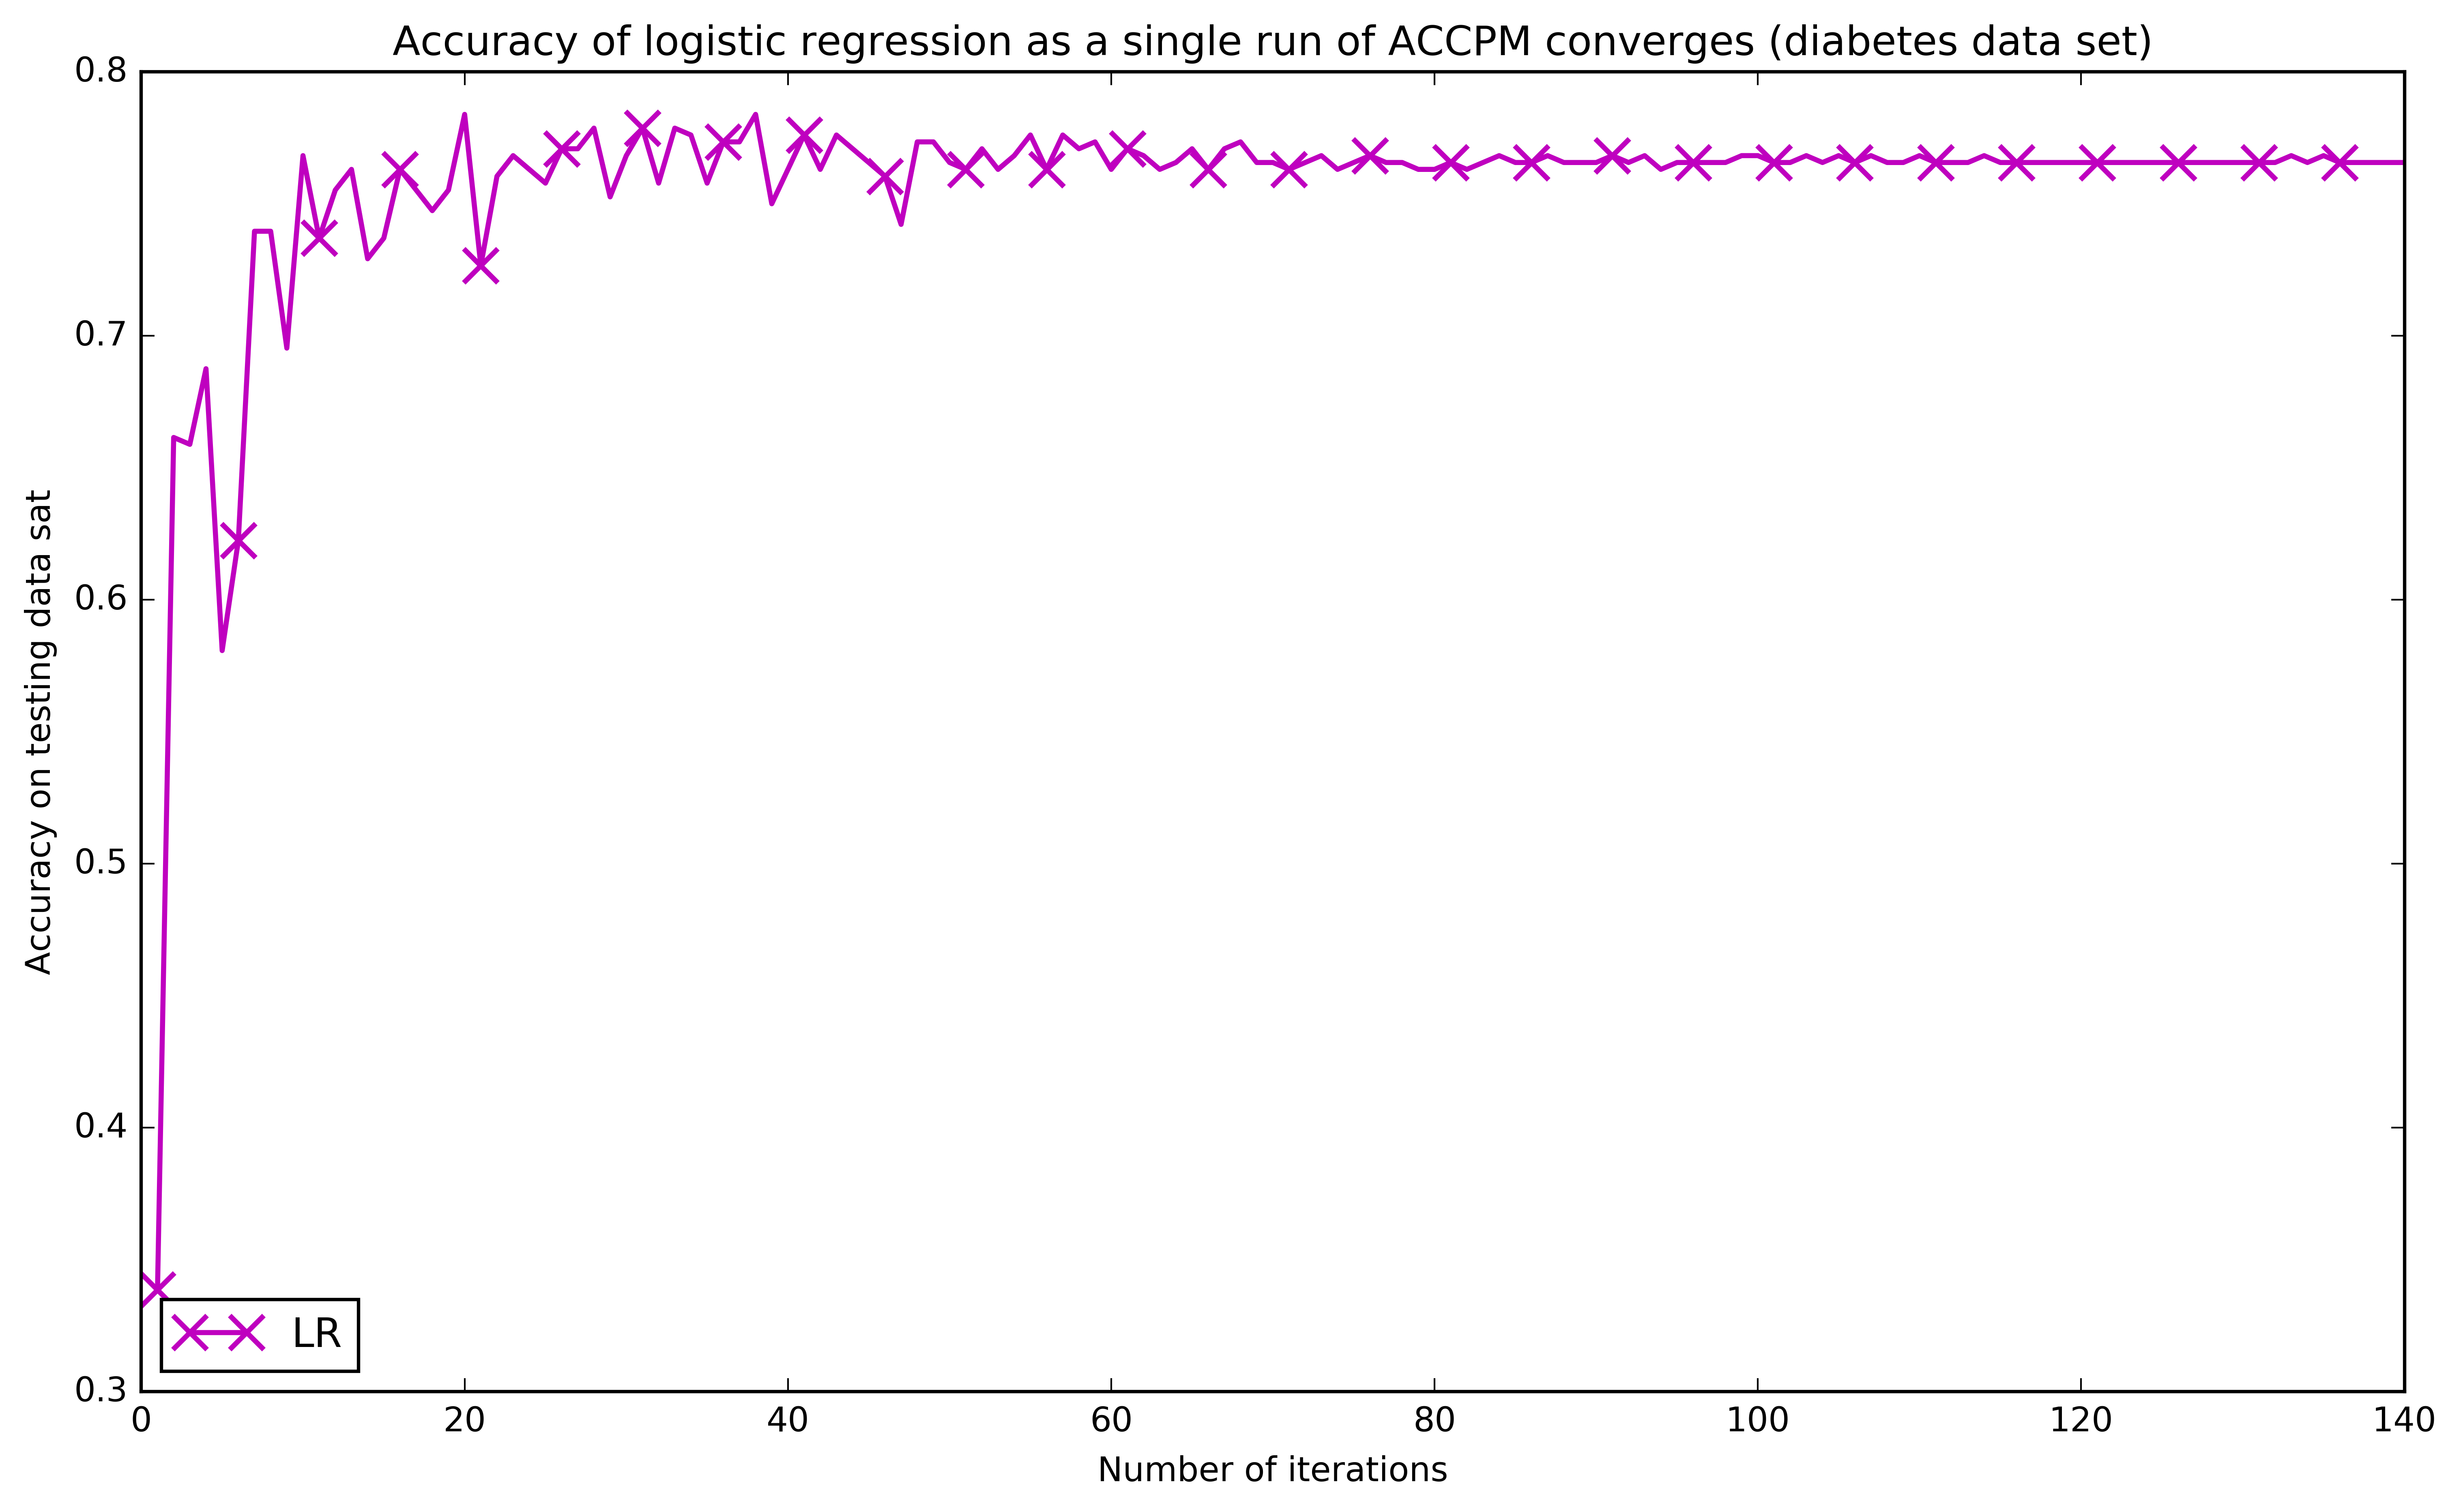
\includegraphics[width=\linewidth]{figures/accpm_experiment.png}
        \end{figure}  
        \FloatBarrier

    \subsection{Discussion of ACCPM experiment}
        The ACCPM successfully converged after 140 iterations. It is re-assuring to know that the ACCPM performed as well as using the model trained using $\texttt{scipy.optimize}$, in both cases achieving an upper-bound of 75\% accuracy. Indeed, we see that convergence in accuracy was rapid, which matches our intuition that as the polyhedron becomes smaller, the points within it should be more accurate parameter vectors. 

        It is interesting to observe that accuracy reached its upperbound well before the stopping criterion was satisfied.

    \subsection{Active learning experiments} 
        %%%% TO-DO: check the indices in this section are all correct, I think some ones might have to be 0s or vice-versa %%%%
        Our experimental procedure for both data sets is almost the same. Therefore, we explain it using the general set-up introduced in Section \ref{ss:classification} where in total we have $N$ data points. (This is useful also for the reader that might want to replicate these experiments.) 

        The aim of our experimental procedure is to approximate the average change in accuracy from labeling an additional point. To see how we will achive this, we consider a single run of Algorithm \ref{a:active} on the training set $\mathcal{D}_\text{training}$ with the stopping criterion being to label no more than $p$ points. Now, suppose in this single run we label the points such as to produce the sequence $(x_{n_1}, y_{n_1}), (x_{n_1}, y_{n_1}), \dots, (x_{n_{p}}, y_{n_{p}})$. Then at each iteration $i = 0, \dots, p - 1$ we compute a classification vector $w^{(i + 1)}$ which is associated with the sequence of labeled points $(x_{n_1}, y_{n_1}), (x_{n_2}, y_{n_2}), \dots, (x_{n_{i}}, y_{n_{i}})$. For each $i = 1, \dots, p$ we can then test the predictions of $f_{w^{(i)}}$ against $\mathcal{D}_\text{testing}$ to compute an accuracy $r^{(1)}_i \in [0, 1]$. (The reason for the upper-index will be made clear shortly.) Now, as choosing the point to be labeled involves a random process, each time we run the algorithm we may produce a different sequence of weights $w_1, \dots, w_p$. Therefore, we run the algorithm $q$ times and the run we are up to is indicated by the upper-index. Doing this we produce a $q \times p$ matrix of accuracies
        \begin{equation*}
            R \coloneqq \begin{bmatrix}
            r_1^{(1)} &  r_2^{(1)}  & \cdots & r_p^{(1)}\\
            r_1^{(2)}  &  r_2^{(2)} & \cdots & r_p^{(2)}\\
            \vdots & \vdots & \ddots & \vdots\\
            r_1^{(q)}  &  r_2^{(q)}  & \cdots & r_p^{(q)}
            \end{bmatrix}.
        \end{equation*}
        The average accuracy $r_i$ of the algorithm when $i = 1, \dots, p$ points have been labeled can then be computed as
        \begin{equation*}
            r_i \coloneqq \frac{r_i^{(1)} + \dots + r_i^{(q)}}{q}.
        \end{equation*}
        (That is, the average computed over the $i$-th column.)

        We complete this procedure of running the Algorithm \ref{a:active} $10$ times, labeling 25 points each time, and computing $r_1, \dots, r_p$ three times in total; one each for the query point each iteration being computed as (i) the CC; (ii) the AC; and (iii) a randomly chosen point of the current iteration's candidate space. 

        We also analogously complete this process for logistic regression, for purposes of comparison, where for a single run (out of 10) at the $1$-th iteration we randomly select a data point $(x_{n_1}, y_{n_1})$ from $\mathcal{D}_\text{training}$ without replacement. We then train logistic regression on the data point $(x_{n_1}, y_{n_1})$ and use the resultant model and testing data set $\mathcal{D}_\text{testing}$ to produce a accuracy $r_0^{(1)}$. On the $2$-th iteration we again randomly select another data point $(x_{n_1}, y_{n_1})$ from $\mathcal{D}_\text{training}$ without replacement. We then train logistic regression on the data points $(x_{n_1}, y_{n_1}), (x_{n_2}, y_{n_2})$ and use the resultant model and testing data set $\mathcal{D}_\text{testing}$ to produce an accuracy $r_1^{(1)}$. We do this for $24$ iterations. We then repeat this another 9 times to produce the matrix $R$ from which $r_1, \dots, r_p$ can be computed.

        In the experiment using the Iris flower data set we label $p = |\mathcal{D}_\text{training}| = 75$ data points each run and run the algorithm $q = 10$ times. 

        In the experiment using the diabetes data set we label $p = 15$ data points each run and run the algorithm $q = 10$ times. 

        For the experiment using the diabetes data set we also computed (i) the average accuracy of logistic regression trained on half of the points from $\mathcal{D}_\text{training}$, computed by averaging over 10 runs of training logistic regression on a randomly selecting subset of $\mathcal{D}_\text{training}$ that is half the size of $\mathcal{D}_\text{training}$; and (ii) the accuracy from training logistic regression on the entire training data set $\mathcal{D}_\text{training}$

        We used our own implementation of logistic regression where the training is completed using the $\texttt{scipy.optimize.minimize(method='BFGS')}$ function. It is worth noting that when computing the classification vector for logistic regression the minimization function  often failed to converge, although it would still produce a classification vector. We went ahead and used these classification vectors.

        \subsection{Implementation details} The notebooks corresponding to these experiments can be found in the GitHub repository in \texttt{experiment\_active\_iris.ipynb} and \texttt{experiment\_active\_diabetes.ipynb}. 

        \newpage
        \begin{figure}[h]
            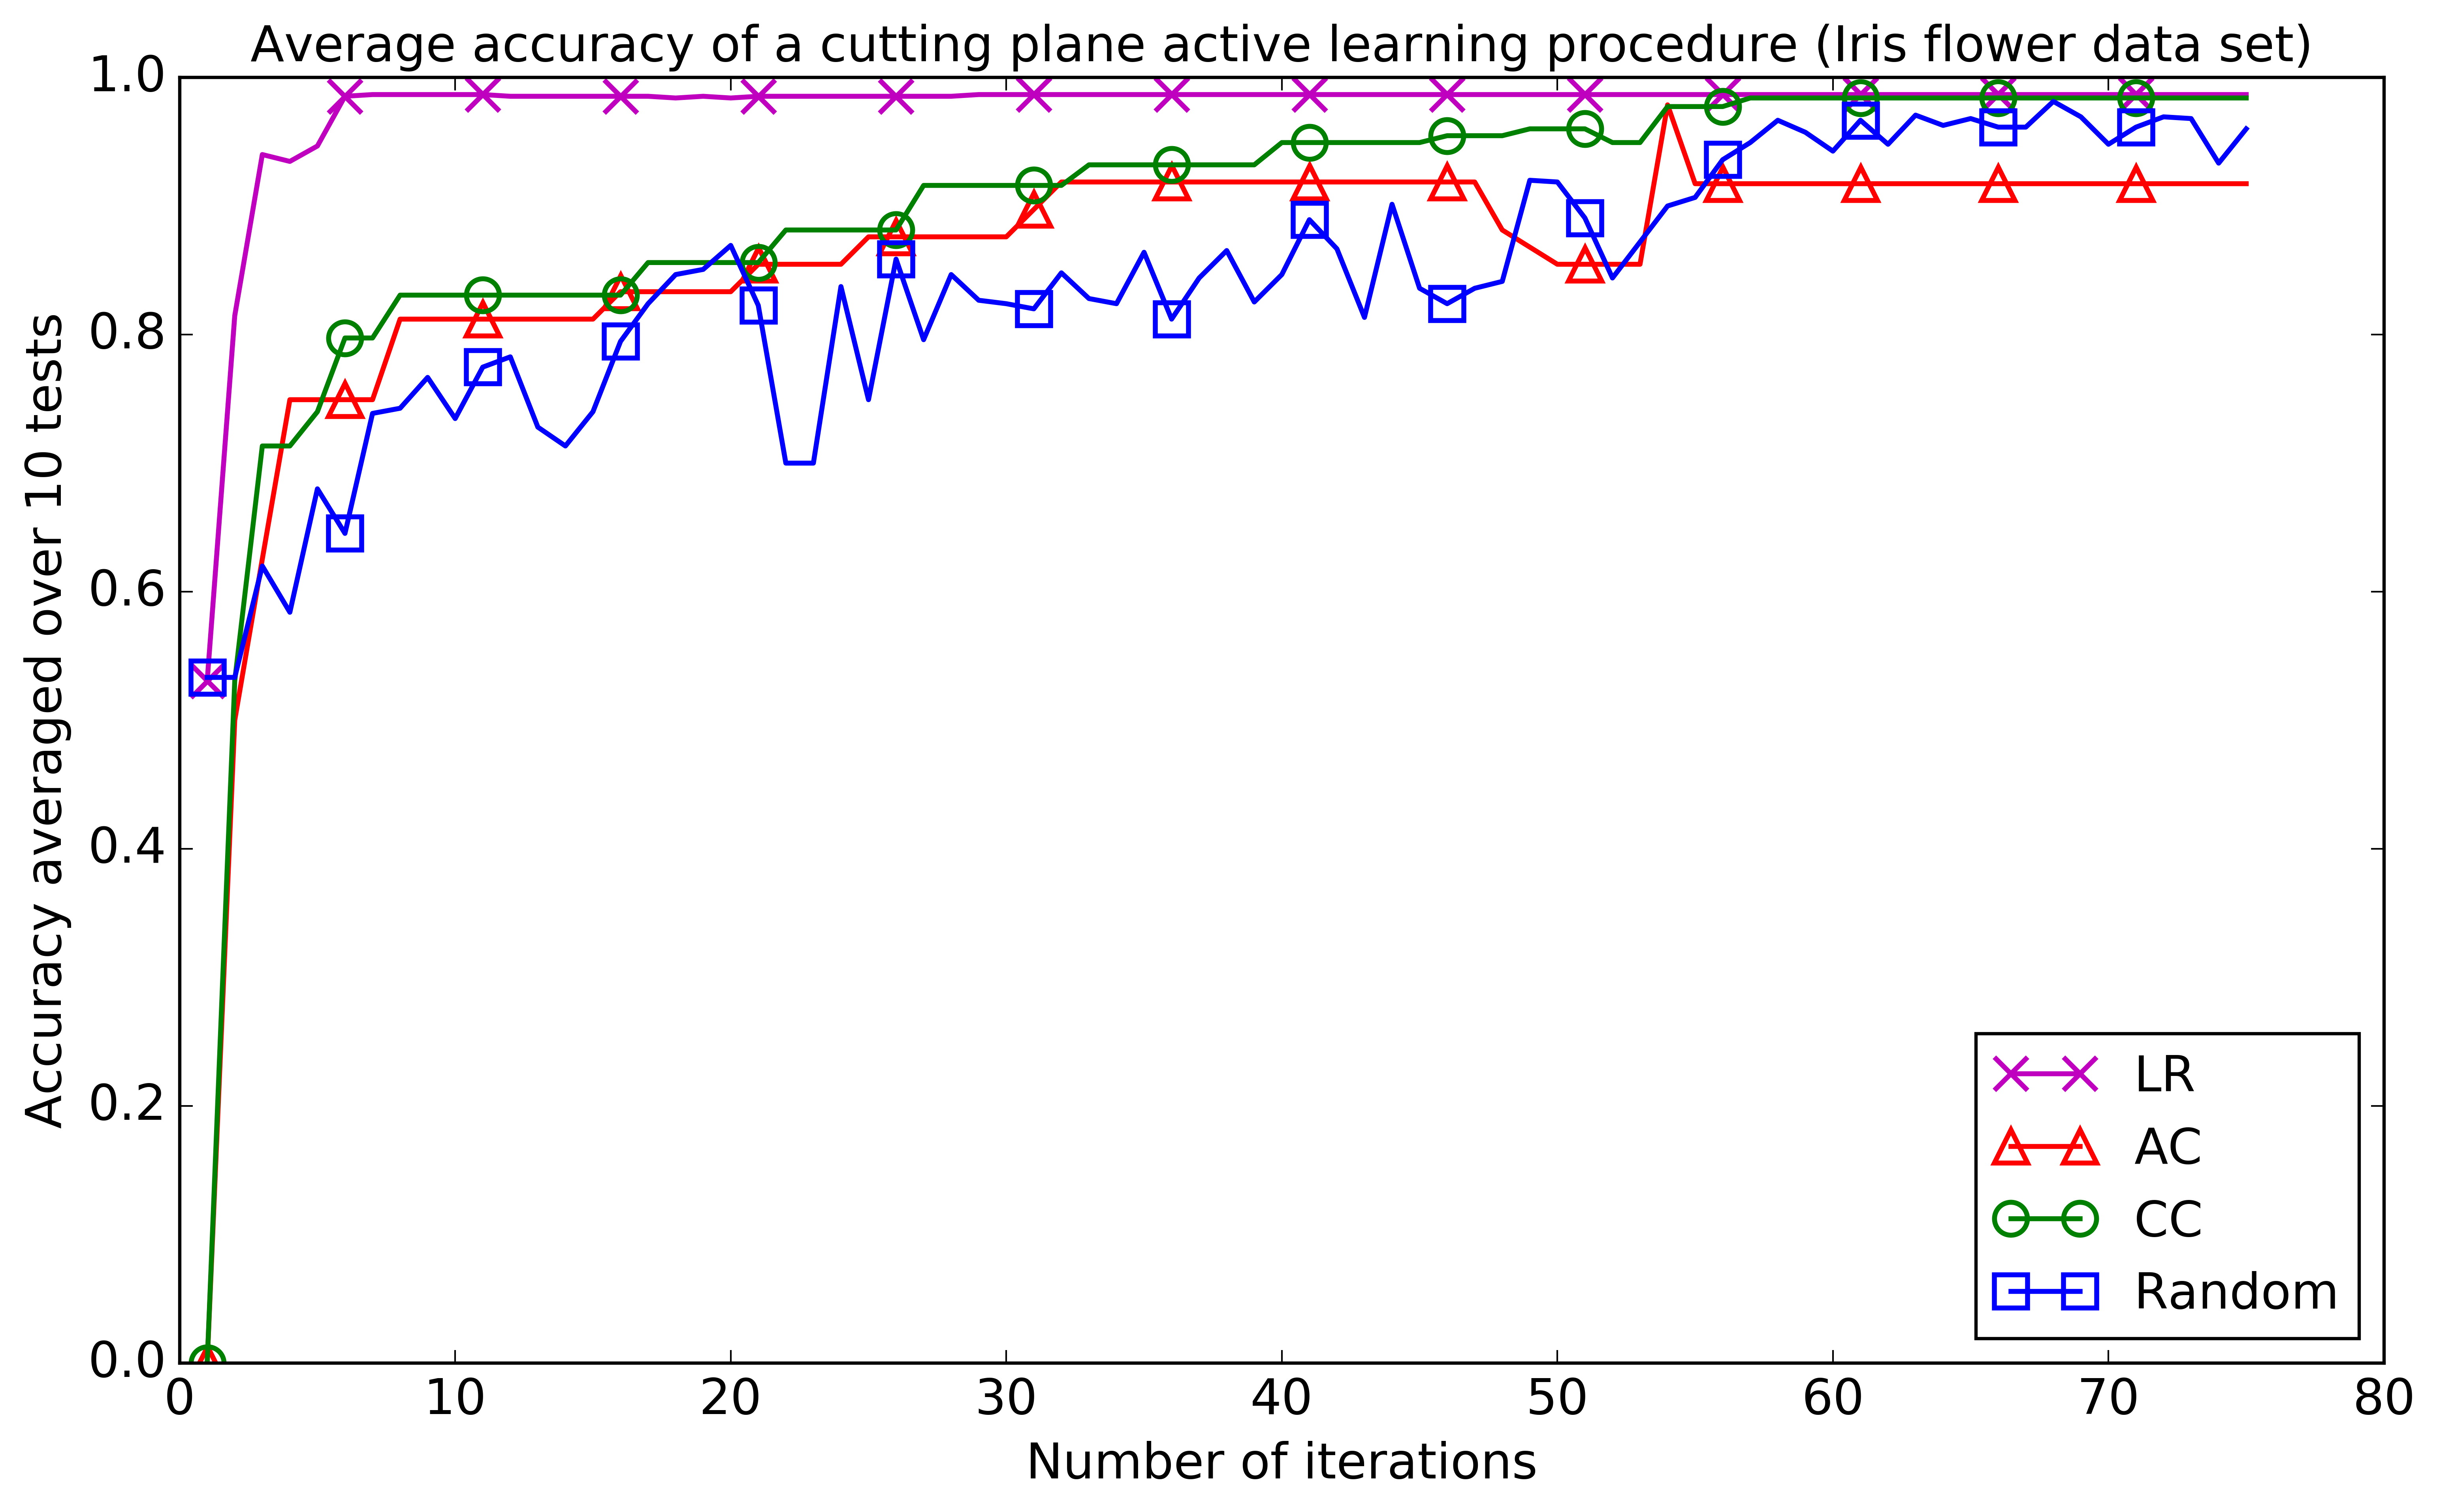
\includegraphics[width=\linewidth]{figures/iris_experiment.png}
            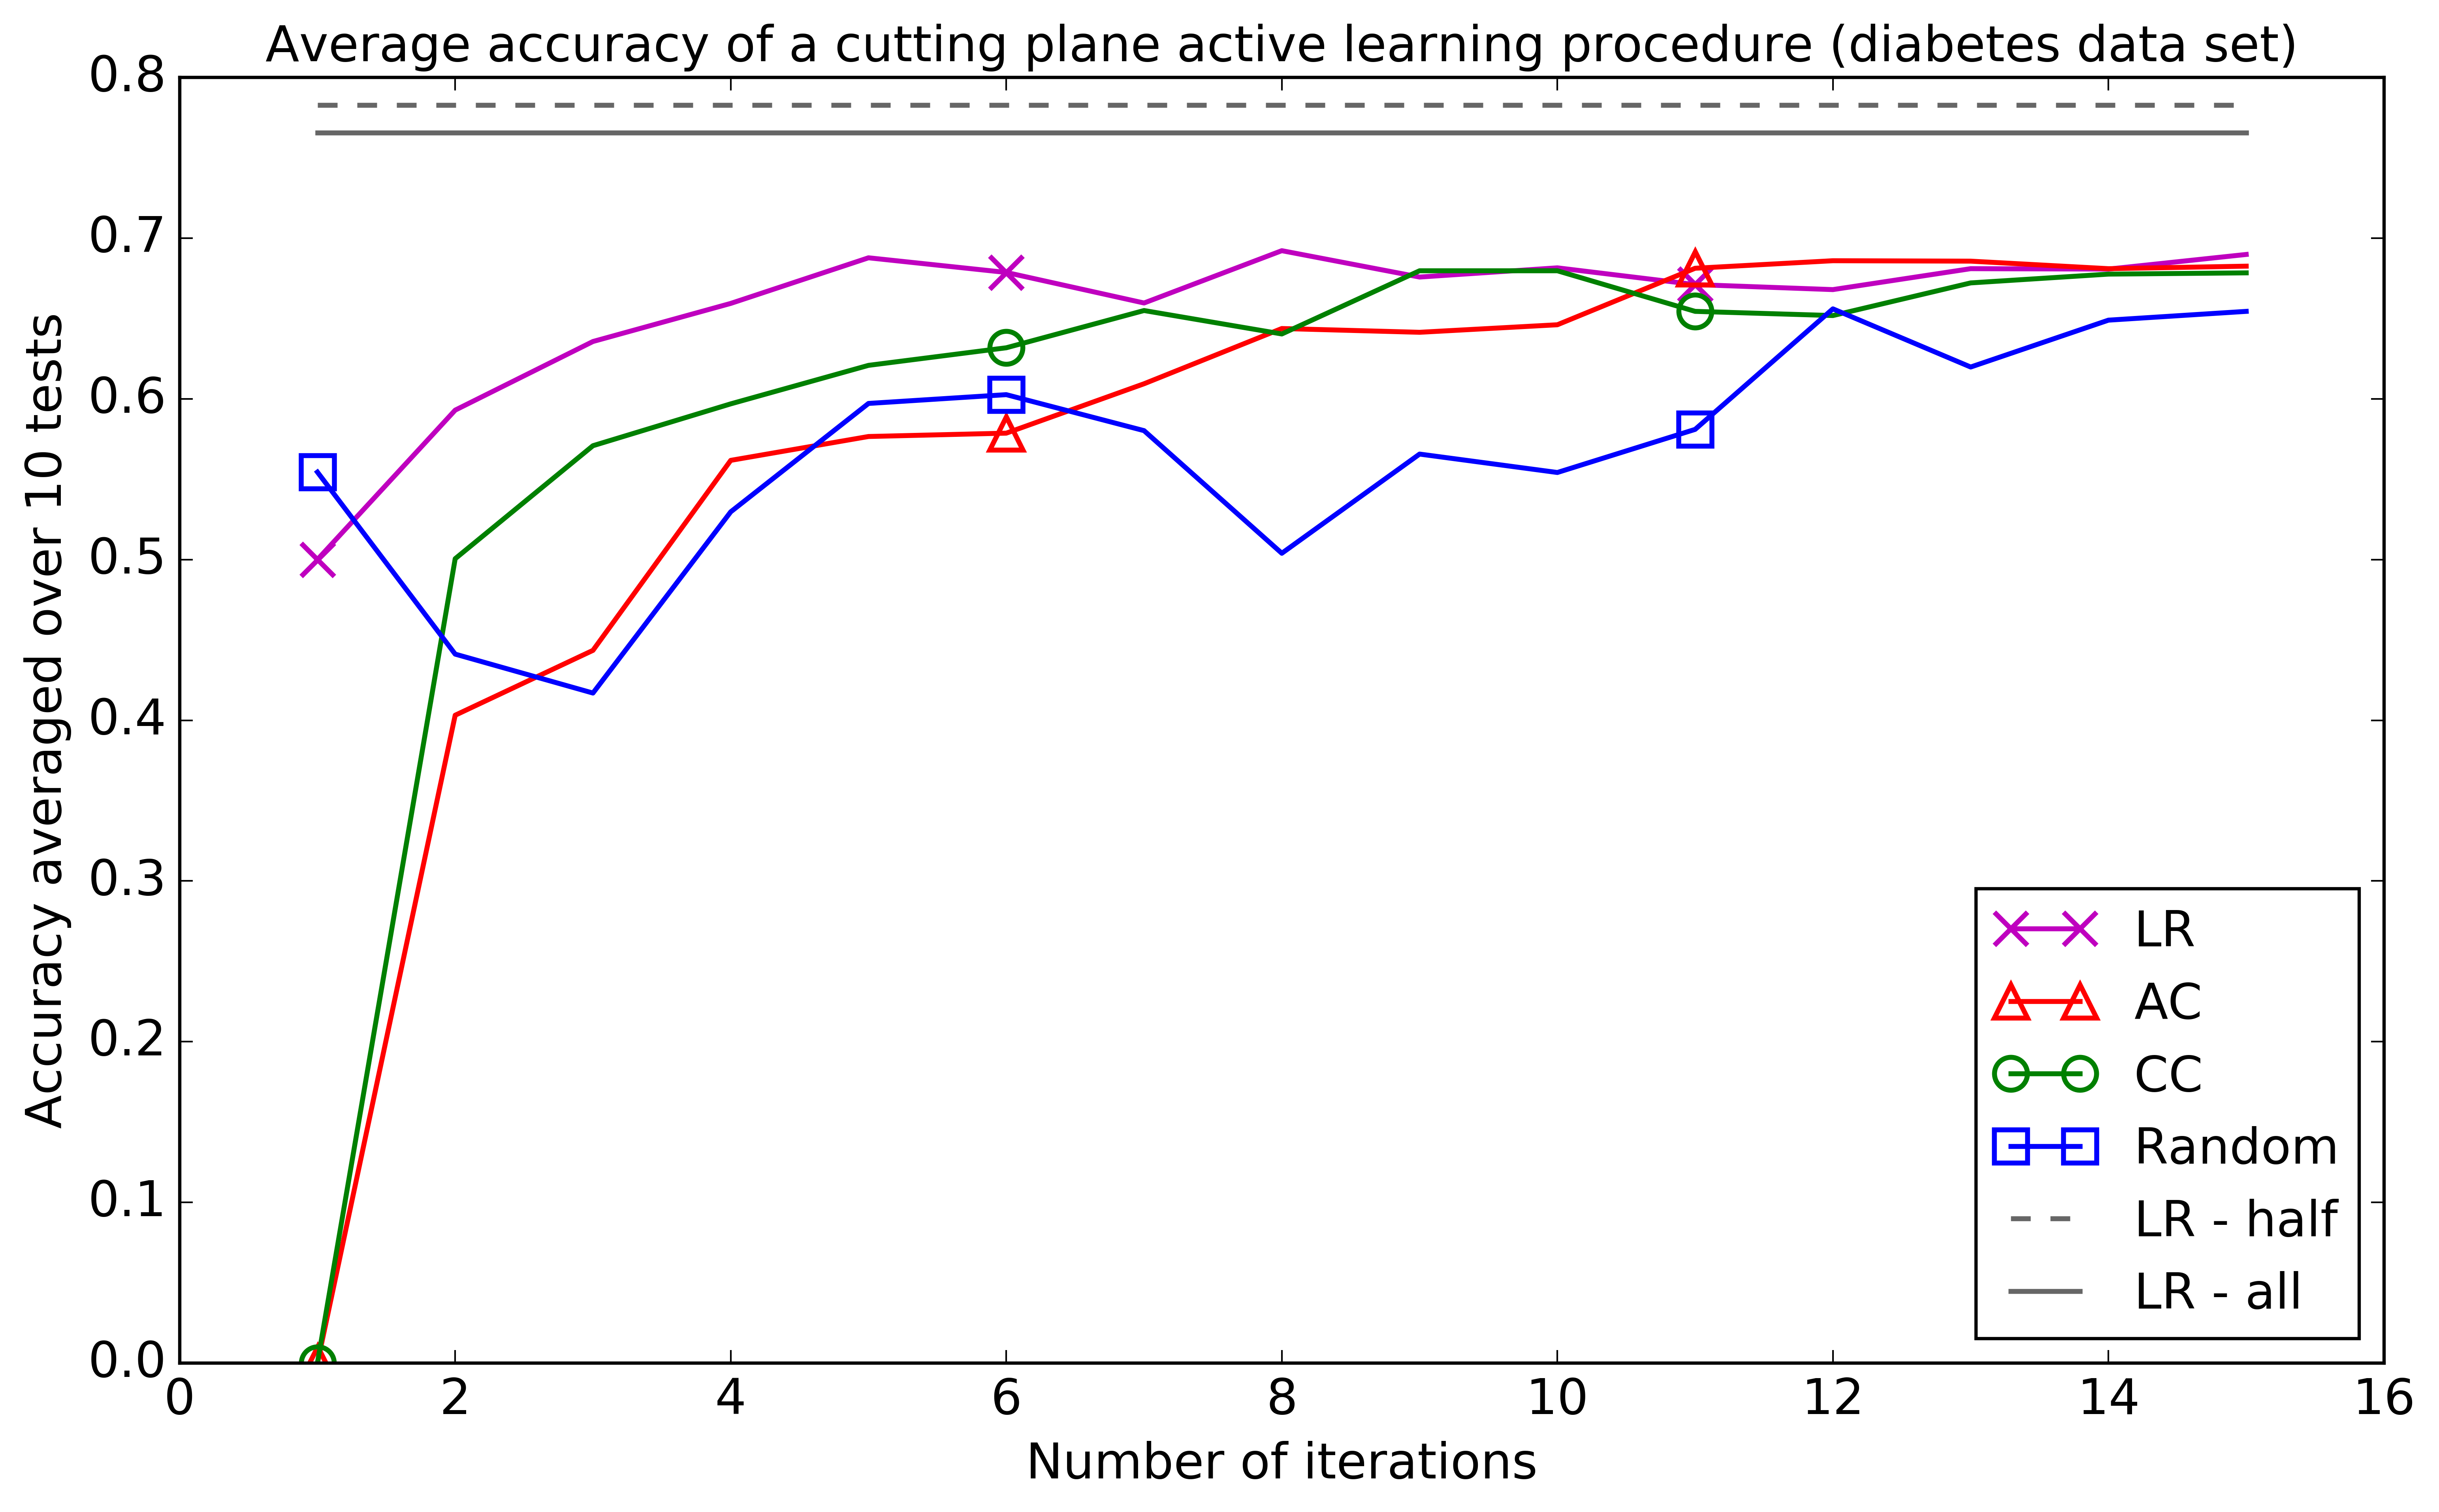
\includegraphics[width=\linewidth]{figures/diabetes_experiment.png}
        \end{figure}
        \newpage

    \subsection{Discussion of active learning experiments}
        In both the experiment on the Iris flower data set and the diabetes data set we see that our implementation of logistic regression (LR) trained on a random sample outperformed the active learning algorithm with query point as the AC (AC), CC (CC) and random center (Random). In Section \ref{s:conc} we will give suggestions on how the performance of the active learning algorithm could be improved.

        In the experiment with the Iris flower data set we see that overall CC outperformed AC and Random and performed on par with LR after approximately $55$ iterations. AC performed similarly to CC, and outperformed Random with the exception that after aproximately $45$ iterations the average accuracy of AC dropped signficantly. 

        Although we have not investigated this, it is possible that this can be attributed to a numerical computing error occurring once the candidate space $\mathcal{C}_k$ becomes very small. This seems a reasonable cause given that the implementation of the AC computation was our own and numerical computing issues did arise during its development. Consistent with this, the smoother behavior of CC could be in part due to relying on the robust \texttt{scipy.optimize.linprog} function to compute the CC. 

        In the experiment with the diabetes data set we first observe that on average logistic regression trained on half the training data set (LR-- half) and the whole training data set (LR--all) performed the best but still with average accuracy less than 80\%. Indeed, it is interested to observe that LR--half outperformed LR--all, which could possibly be attributed to the data set not being linearly separable. Like the experiment on the Iris flower data set we see that AC and CC outperformed random and CC outperformed AC.

        LR significantly outperformed AC and CC on the Iris flower data set and while it also outperformed AC and CC on the diabetes data set this was not as significantly and after roughly $9$ iterations, LR, AC and CC performed approximately equally. 

        In regards to the experiment on the diabetes data set, it is worth noting that we only included data up to labeling at most $15$ points as the computation time grew exponentially with the maximum number of points to be labeled. Having said this, there is partial data for labeling at most $30$ points, which took approximately $36$ hours to compute. For the interested reader, this can be found in the GitHub repository. This running time growth can be attributed to using rejection sampling to sample the points in the \textsc{Query} function. Specifically, random vectors were drawn from a nine-dimensional unit hypercube centered at the origin and were rejected if they did not lie in the current candidate space $\mathcal{C}_k$. We remark that it is known that as the dimension increases, rejection sampling tends to perform exponentially worse. We see this in how computing each of AC, CC and Random in the case of labeling at most $15$ points involved generating at least $1, 000, 000$ random vectors while the case of labeling at most $30$ points involved generating at least $1, 000, 000, 000$ random vectors.

\section{Conclusion}\label{s:conc}
    In this report we showed how a general cutting-plane algorithm can be specialized for the purposes of convex optimization and an active learning problem. This specialization involves specifying (i) the target set; (ii) how query points are chosen; (iii) how cutting-planes are constructed; and (iv) stopping criterion. And as we saw in the case of the active learning problem, these choices effect the performance of the algorithm. Now, the experiments on both the Iris flower data set and diabetes data set LR outperformed both the CC and AC based cutting-plane algorithms. This raises the general question of what options there are to improve the performance of a cutting-plane algorithm? (Specifically, the question I am interested in is what can be done to improve the performance of the active learning algorithm.) In their 2011 notes S. Boyd and L. Vandenberghe \cite[Section 5]{BV11} provide a number of suggestions for extending the general cutting-plane algorithm:
    \begin{enumerate}
        \item each iteration instead of returning a single cutting-plane, we can return \emph{ multiple} cutting-planes;
        \item each iteration we can remove (or in other words \emph{drop} or \emph{prune}) inequality constraints that may be redundant;
        \item we can limit the number of inequality constraints; and
        \item we can allow \emph{non-linear} cuts.
    \end{enumerate}
    In our implementation we did not include any of these extensions. Of particular promise is the suggestion to limit the number of inequality constraints as it is suggested that this can lead to improved accuracy iteration-by-iteration \cite[Section 5]{BV11}. Therefore, we see that the general cutting-plane algorithm is a highly adaptable algorithm.

\renewcommand\refname{Bibliography}
\begin{thebibliography}{99}
    \bibitem[Bis06]{Bis06} C. Bishop. \emph{Pattern Recognition and Machine Learning}. Springer, 2006.
    \bibitem[BV04]{BV04} S. Boyd and L. Vandenberghe. \emph{Convex Optimization}. Cambridge University Press, 2004.
    \bibitem[BVS08]{BVS08} S. Boyd, L. Vandenberghe and J. Skaf. \emph{Analytic Center Cutting-Plane Method}. 2008. \url{https://see.stanford.edu/materials/lsocoee364b/06-accpm_notes.pdf}.
    \bibitem[BV11]{BV11} S. Boyd and L. Vandenberghe. \emph{Localization and Cutting-Plane Methods}. 2011. \url{http://web.stanford.edu/class/ee364b/lectures/localization_methods_notes.pdf}.
    \bibitem[BDV15]{BDV15} S. Boyd, J. Duchi and L. Vandenberghe. \emph{Subgradients}. 2015. \url{http://web.stanford.edu/class/ee364b/lectures/subgradients_notes.pdf}.
    \bibitem[Das11]{Das11} S. Dasgupta. (2011). Two faces of active learning. \emph{Theoretical Computer Science}, Volume 412, Issue 19, pp. 1767-1781.
    \bibitem[LR15]{LR15} U. Louche and L. Ralaivola. (2015). From Cutting Planes Algorithms to Compression Schemes and Active Learning. \emph{2015 International Joint Conference on Neural Networks}, pp. 1-8.  
\end{thebibliography}

% Examples:
% \bibitem[AHU]{ahu} Aho, A.,\ Hopcroft, J.,\ and Ullman, J.\ (1976). {\em{The Design and Analysis of Computer Algorithms.}} Addison Wesley, Reading, Mass.

% \bibitem[AT]{AT} Auslander, L. and Tolmieri, R. (1979). Is Computing with the Fast Fourier Transform Pure or Applied Mathematics? {\em{Bulletin (New Series) of the AMS Vol. 1}} 847-897.

% [Lee03] John Lee, \emph{Introduction to Topological Manifolds}, Springer Science, New York, USA, 2003.

% [Rat06] John Ratcliffe, \emph{Foundations of Hyperbolic Manifolds}, Springer Science, New York, USA, 2006.

\end{document}